\documentclass[a4paper]{article}

\usepackage[english]{babel}
\usepackage[utf8x]{inputenc}
\usepackage{amsmath}
\usepackage{graphicx}
\usepackage{unicode-math}
\usepackage{bbold}
\usepackage[colorinlistoftodos]{todonotes}

\title{ECE276A Project 1: Orientation Tracking}
\author{Awies Mohammad Mulla}

\begin{document}
\maketitle

\begin{abstract}
As we know an Inertial Measurement Unit (IMU) is one of the basic sensor used in the field of Robotics (in Autonomous Navigation, Bio-mimetic robots, and even in our smartphones for various applications; from using navigation to capturing wide images called panorama). In this project we attempt to use the given Inertial Measurement Unit Datasets to estimate the pose of the body i.e. camera and clip together the snapshots captured by camera different instances to generate an image called panorama.
\end{abstract}

\section{Introduction}
We are provided with the datasets of different sensors i.e. Inertial Measurement Unit (IMU), wheel encoders,2D LIDAR Scanner, and RGBD camera (kinect). We will be estimating the robot pose throughout the dataset using the readings from IMU and encoder. From LiDAR scans we obtain the coordinates of obstacle present in LiDAR's frame. The range of given LiDAR is -135 to 135 degree. We will use these scans to plot occupancy grid map. We are provided with disparity and RGB images (480 x 640) from the Kinect. The specifications of the camera are mentioned later int he report. These images will be used to genrate a texture map of the environment to get more information about the environment in which the robot is operating.

Our goal is to generate an occupancy grid map of area where dataset was collected and also to simultaneuosly estimate the pose of robot throughout the traversal, using the readings from IMU, wheel encoders and LIDAR. We would be building a texture map using the estimated SLAM pose and images from obtained from kinect. Problem of SLAM is essential to navigate an unmanned vehicle in an unknown environment. The mentioned problem is an essential building block in SLAM as, currently, we are using the most basic sensors (which can be mounted on any robot) to achieve this goal. The approach described in this report can be extrapolated to navigate the robot in more complex environments. For example: we can also use 3D Velodyne LiDAR scanner to get the pointcloud of the environment and navigate the robot more effectively. On top  of that texture map gives us generic idea of the environment in which robot is operating.

We will be using the readings from gyroscope of IMU to estimate the yaw rate of the robot and readings from wheel encoders to estimate the linear velocity of the robot. To obtain the robot pose we will use Euler's discrete-time kinematics model with linear and angular velocity mentioned above. We will use this pose along with the LiDAR scans obtained to generate occupancy grid map using a particle filter. The particle filter consists of a motion and observation model. The motion model predicts the robot pose at next timestep and observation model corrects this pose and extends the map. This is carried out by sampling and exploring N particles. Now our goal is streamlined to find most accurate robot pose given the current poses of particles and map. This pose will then be used to extend our occupancy grid map. Later, we will be using this pose for transforming and projecting the images obtained from kinect onto the map.
\subsection{Frame Conventions}
The robot heading is defined zero when robot heading towards the positive x-axis. So, the lidar scans are also defined in similar manner. The occupancy grid map obtained would 90 degree clockwise rotated with respect to previous convention. Since, it was only rotated (instead of mirrored about any axis or line) we did not reorder to plot the m. The texture map also follows this convention.
\section{Problem Formulation}
Our goal is to generate an occupancy grid map using the datasets provided. We will be implementing the particle filter to generate the map. And using the poses obtained from the particle filter, we will be generating a texture map using the images given.
\subsection{Particle Filter}
\begin{enumerate}
    \item Each particle (i) is a hypothesis that the value of robot pose $s_t$ is $\mathbf{x}_{i}$ with the probability $w_{i}$.
    \item The particle filter uses the particles with locations $\mathbf{x}_{i}$ and weights $w_{i}$ to represent the posterior distributions of the robot pose $s_t$.
    \begin{equation}
        p_{t|t}(s_t) = \sum_{i=1}^{N} w_{i,t|t} \delta(s_t - \mathbf{x}_{i,t|t})
    \end{equation}
    \item Our goal is to estimate the above distribution at every time step $t$ and generate the occupancy grid map, by estimating the probability mass $p(\mathbf{m}| \mathbf{z}_{0:t}, \mathbf{x}_{0:t})$ (where $\mathbf{m}$ is the map and $\mathbf{z}_{0:t}$ is the set of observations from the sensors).
    \item To estimate the state distributions of the robot we will be plugging the above distribution in the Bayes' filter prediction and update steps.
    \item Prediction step: Let $\mathbf{x}_{i,t+1|t} ~ p_f(.|\mathbf{x}_{i,t|t}, \mathbf{u}_{t})$ and $w_{i,t+1|t} = w_{i,t|t}$, we get:
    \begin{equation}
        p_{t+1|t}(s_{t+1}) \approx \sum_{i=1}^{N} w_{i,t+1|t} \delta(s_{t+1} - \mathbf{x}_{i,t+1|t})
    \end{equation}
    \item Update step: Rescaling the hypothesized probabilities of the poses based on the observation model, we get:
    \begin{equation}
        p_{t+1|t+1}(s_{t+1}) = \sum_{i=1}^{N} w_{i,t+1|t+1} \delta(s_{t+1} - \mathbf{x}_{i,t+1|t+1})
    \end{equation}
    where, $w_{i,t+1|t+1} = frac{w_{i,t+1|t} p(\mathbf{z}_{t+1}|\mathbf{x}_{i,t+1|t})}{k}$, with $k$ as a normalization constant.  $p(\mathbf{z}_{t+1}|\mathbf{x}_{i,t+1|t})$ is the observation model, which here is the likelihood of the LiDAR scan given the pose of the robot.
    \item In the Updated step only the weights of the particles are updated. The particles are not updated.
    \item Now we will be using the LiDAR likelihood distribution of highest weight particle to generate the occupancy grid map as:
    \begin{equation}
        p(\mathbf{m}| \mathbf{z}_{0:t}, \mathbf{x}_{0:t}) \propto p(\mathbf{z}_{t+1}|\mathbf{x}_{i,t+1|t})
    \end{equation}
    \item Resampling: If the weights of certain particles are less than a threshold ($w_i{t+1|t+l} < \frac{1}{4N}$), we will resample the particles.
    \item We will carry above mentioned steps for every time step to estimate most probable distribution.
\end{enumerate}
\subsection{Texture Mapping}
Our goal here is to generate a texture map of the environment using the images obtained from kinect. Obtain the depth of each RGB pixel using the disparity image. Transform these pixels to world frame coordinates and project them onto a map to obtain required texture map.
\section{Technical Approach}
\subsection{Preprocessing sensor data}
As we know, each sensor has its own frequency, and, hence the sensor data is not synchronized. We are provided with the unix timestamps, which we will be using to synchronize the data from different sensors. Given two sensors with different frequencies, we will be sampling in terms of the sensor whose time difference is higher or in other words whose frequency is lower. Hence, given the frequency of wheel encoders (40Hz) and IMU (100Hz), we will sample the data from IMU such that timestamps from IMU and encoders approximately match (here error taken as 0.01 seconds). We could have also extrapolated the data from the encoders to match the frequency of IMU, but in this approach we would be assuming a specific motion of the robot between two datapoints of encoders, which might cause errors. Hence, we decided to synchronize the data with respect to sensor of low frequency. We will carry out similar synchronization approach to synchronize data from LiDAR and encoders.

As mentioned in the problem statement, the timestamps obtained from kinect are somewaht irregular, we will use a slightly different approach while plotting texture map. We will simply look through all the obtained SLAM poses timestamps and choose the one which is closest to the current image (which is being processed) timestamps.
Since IMU data is noisy, we will be passing the gyroscope readings through a low pass filter to remove the noise. We will be using a simple first order low pass filter, which is given by:
\begin{equation}
y(t) = \alpha x(t) + (1-\alpha) y(t-1)
\end{equation}
where $x(t)$ is the input signal, $y(t)$ is the output signal, $\alpha$ is the filter coefficient and $t$ is the time. We will be using $\alpha = 0.1$ for this project. We obtained the filter coefficient from the following formula:
\begin{equation}
\alpha = \frac{2\pi f_c}{2\pi f_c + 1}
\end{equation}
where $f_c$ is the cut-off frequency. We will be using $f_c = 10Hz$ for this project.

\subsection{Motion Model}
The motion model used in this project is a 2D Euler discretization of Differential-drive kinematics model. The model is given by:
\begin{equation}
\begin{bmatrix}
x_{t+1} \\
y_{t+1} \\
\theta_{t+1}
\end{bmatrix} = \begin{bmatrix}
x_t \\
y_t \\
\theta_t
\end{bmatrix} + \begin{bmatrix}
v_t \cos(\theta_t) \\
v_t \sin(\theta_t) \\
\omega_t
\end{bmatrix} \Delta t
\end{equation}
where $x_t, y_t, \theta_t$ are the position and orientation of the robot at time $t$, $v_t$ is the linear velocity of the robot at time $t$, $\omega_t$ is the angular velocity of the robot at time $t$ and $\Delta t$ is the time difference between time $t$ and time $t+1$. We will be using the IMU's gyroscope data for angular velocities of the robot, and the wheel encoders for linear velocities of the robot. The linear velocity of the robot is given by:
\begin{equation}
v_t = \frac{v_R + v_L}{2}
\end{equation}
where $v_R$ is the right wheel velocity and $v_L$ is the left wheel velocity. The right and left wheel velocities are given by:
\begin{equation}
v_R = \frac{\pi dz_{R}}{\Delta t \ 360}
\end{equation}
\begin{equation}
v_L = \frac{\pi dz_{L}}{\Delta t \ 360}
\end{equation}
where $d$ is the diameter of the wheel, $z_{R}$ is the average encoders count of the right wheel and $z_{L}$ is the average encoders count of the left wheel. Given $d = 0.254m$. The representation of the encoder counts is mentioned in the problem statement. 

\subsection{Occupancy Grid Mapping}
Our goal is to generate a 2D occupancy grid map $(\mathbf{m})$ of the environment given the robot trajectory $\mathbf{x}_{0:t}$ and sequence of LiDAR scans $\mathbf{z}_{0:t}$. Since the map is unknown and the measurements are uncertain, we maintain a probability mass $p(\mathbf{m}| \mathbf{z}_{0:t}, \mathbf{x}_{0:t})$ for each cell in the map. We will assume each cell values to be independent of each other, hence the probability mass for each cell is given by:
\begin{equation}
p(\mathbf{m}| \mathbf{z}_{0:t}, \mathbf{x}_{0:t}) = \prod_{i=1}^{N} p(\mathbf{m}_i| \mathbf{z}_{0:t}, \mathbf{x}_{0:t})
\end{equation}
where $N$ is the number of cells in the map.

Modelling the map cells as Bernoulli random variables, we get
\begin{equation}
    m_i = \begin{cases}
    1 & \text{(if cell is occupied)} \ with \ probability \ \gamma_{i,t} = p( \mathbf{m}_i = 1| \mathbf{x}_{0:t}, \mathbf{z}_{0:t}) \\
    -1 & \text{(if cell is free)} \ with \ probability \ (1-\gamma_{i,t})
    \end{cases}
\end{equation}
where $\gamma_i$ is the probability of the cell being occupied. We will be using the Bayes rule to update the probability of the cell being occupied given the LiDAR scan and the robot pose. The Bayes rule is given by:
\begin{equation}
\begin{aligned}
    p(\mathbf{m}_i| \mathbf{z}_{0:t}, \mathbf{x}_{0:t}) &= \frac{1}{k}p(\mathbf{z}_{t} | \mathbf{x}_{t}, \mathbf{m}_i = 1) p(\mathbf{m}_i = 1 | \mathbf{z}_{0:t-1}, \mathbf{x}_{0:t-1}) \\
    &= \frac{1}{k}p(\mathbf{z}_{t} | \mathbf{x}_{t}, \mathbf{m}_i = 1) \gamma_{i,t-1}
\end{aligned}
\end{equation}
where $k$ is a normalizing constant. Odds ratio of Bernoulli random variable ($o(m_i | \mathbf{z}_{0:t}, \mathbf{x}_{0:t})$) $m_i$ is given by:
\begin{equation}
\begin{aligned}
    \frac{p(\mathbf{m}_i = 1 | \mathbf{z}_{0:t}, \mathbf{x}_{0:t})}{p(\mathbf{m}_i = -1 | \mathbf{z}_{0:t}, \mathbf{x}_{0:t})} &= \frac{p(\mathbf{z}_{t} | \mathbf{x}_{t}, \mathbf{m}_i = 1) \gamma_{i,t-1}}{p(\mathbf{z}_{t} | \mathbf{x}_{t}, \mathbf{m}_i = -1) (1-\gamma_{i,t-1})} \\
    &= \frac{p(\mathbf{z}_{t} | \mathbf{x}_{t}, \mathbf{m}_i = 1) \gamma_{i,t-1}}{p(\mathbf{z}_{t} | \mathbf{x}_{t}, \mathbf{m}_i = -1) (1-\gamma_{i,t-1})} \\
    &= \frac{p(\mathbf{z}_{t} | \mathbf{x}_{t}, \mathbf{m}_i = 1)}{p(\mathbf{z}_{t} | \mathbf{x}_{t}, \mathbf{m}_i = -1)} \frac{\gamma_{i,t-1}}{1-\gamma_{i,t-1}}
\end{aligned}
\end{equation}
where $p(\mathbf{z}_{t} | \mathbf{x}_{t}, \mathbf{m}_i = 1)$ is the probability of the LiDAR scan given the robot pose and the cell being occupied. The Observation model odds ratio is $g(\mathbf{z}_{t} | \mathbf{x}_{t}, \mathbf{m}_i) \ = \ p(\mathbf{z}_{t} | \mathbf{x}_{t}, \mathbf{m}_i = 1) / p(\mathbf{z}_{t} | \mathbf{x}_{t}, \mathbf{m}_i = -1)$. Simplifying Observation model odds ratio using Bayes Rule, we get:
\begin{equation}
\begin{aligned}
    g(\mathbf{z}_{t} | \mathbf{x}_{t}, \mathbf{m}_i) &= \frac{p(\mathbf{z}_{t} | \mathbf{x}_{t}, \mathbf{m}_i = 1)}{p(\mathbf{z}_{t} | \mathbf{x}_{t}, \mathbf{m}_i = -1)} \\
    &= \frac{p(m_i = 1 | \mathbf{z}_t, \mathbf{x}_t)}{p(m_i = -1 | \mathbf{z}_t, \mathbf{x}_t)} \ \frac{p(m_i = 1)}{p(m_i = -1)} \\
\end{aligned}
\end{equation}
In the above equation, first term represents how much we trust the obtained observation (in the project we assume this ratio as 4 i.e. we assume the obtained scan is 80\% correct). The second term represents the prior probability of the cell being occupied (this can be used when we have some information about the environment). Here we take the prior ratio as 1, since we know nothing about the environment. Now, Odds ratio of occupancy grid mapping is given by:
\begin{equation}
    o(m_i | \mathbf{z}_{0:t}, \mathbf{x}_{0:t}) = o(m_i | \mathbf{z}_{0:t-1}, \mathbf{x}_{0:t-1}) g(\mathbf{z}_{t} | \mathbf{x}_{t}, \mathbf{m}_i) \\
\end{equation}
Log odds ratio of occupancy grid mapping is given by:
\begin{equation}
    \begin{aligned}
        \lambda_{i,t} &= \log o(m_i | \mathbf{z}_{0:t}, \mathbf{x}_{0:t}) \\
    \Delta \lambda_{i,t} &= \log g(\mathbf{z}_{t} | \mathbf{x}_{t}, \mathbf{m}_i)
    \end{aligned}
\end{equation}
Now the updating rule for the log odds ratio (without prior) is given by:
\begin{equation}
    \lambda_{i,t} = \lambda_{i,t-1} + \Delta \lambda_{i,t}
\end{equation}
We will constrain the log odds ratio to be between $-10$ and $10$ to avoid overconfident estimates. The probability of the cell being occupied is given by:
\begin{equation}
    \gamma_{i,t} = \frac{1}{1 + e^{-\lambda_{i,t}}}
\end{equation}
The map for the first scan is shown below:

\begin{figure}[h]
    \centering
    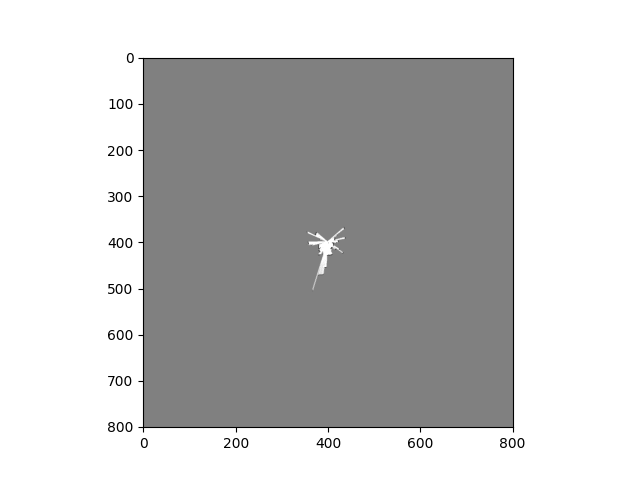
\includegraphics[width=0.5\textwidth]{first_scan.png}
    \caption{Map for the first scan}
    \label{fig:map1}
\end{figure}
\subsection{Observation Model}
The observation model uses the LiDAR scan evaluates the correlation between the scan obtained given the robot pose and the occupancy grid map. To compute the correlation between the scan $\mathbf{z}$ obtained from pose $\mathbf{x}$ and the occupancy grid map $\mathbf{m}$, we first transform the scan to frame of map using appropriate transformation. The transformation is given by:
\begin{equation}
    \begin{bmatrix}
        x_{map} \\
        y_{map} \\
    \end{bmatrix} = \begin{bmatrix}
        \cos(\theta) & -\sin(\theta) \\
        \sin(\theta) & \cos(\theta) \\
    \end{bmatrix} \begin{bmatrix}
        x_{scan} \\
        y_{scan} \\
    \end{bmatrix} + \begin{bmatrix}
        x_{pose} \\
        y_{pose} \\
    \end{bmatrix}
\end{equation}
where $\theta$ is the yaw angle of the robot.
Let $\mathbf{y}$ be the cells in the map that are visible from LiDAR. So, the correlation between the scan and the map is given by:
\begin{equation}
    \text{corr}(\mathbf{y}, \mathbf{m}) = \sum_{i} \mathbb{1}\{\mathbf{y}_i = \mathbf{m}_i\}
\end{equation}
where $\mathbb{1}$ is the indicator function which is 1 if the condition is true and 0 otherwise.
\subsection{Particle Filter}
Sample N particles with pose $\mathbf{x}_{i,0} = [0,0,0]^T$ and weight $w_{i,0} = \frac{1}{N}$. We know that particle filter is Bayes filter where the motion model predicts the next state of the system i.e. $\mathbf{x}_{i,t} = f(\mathbf{x}_{i,t-1}, \mathbf{u}_t)$ and the observation model updates the weights of the particles using the obtained observation i.e. $w_{i,t} = w_{i, t-1} * \text{corr}(\mathbf{y}, \mathbf{m})$. So, each particle represents a hypothesis of the robot pose $\mathbf{x}_{i,t}$ with probability $w_{i,t}$. The implemented particle filter algorithm is given below:
\subsubsection{Prediction Step}
For every particle $i$:
\begin{equation}
    \begin{aligned}
        \mathbf{x}_{i,t} &= f(\mathbf{x}_{i,t-1}, \mathbf{u}_t + \mathbf{\epsilon}_t) \\
        w_{i,t} &= w_{i,t-1}
    \end{aligned}
\end{equation}
\begin{enumerate}
    \item $f(\mathbf{x}_{i,t-1}, \mathbf{u}_t)$ is the Differential-drive motion model (mentioned above).
    \item $\mathbf{u}_t$ is the control input (linear and angular velocity).
    \item $\mathbf{\epsilon}_t$ is the noise in the control input to sample next state of different particles. Here we assume the noise to be Gaussian with mean 0 and covariance matrix $\begin{bmatrix}\sigma_v^2 & 0 \\ 0 & \sigma_\omega^2\end{bmatrix}$. Here $\sigma_v$ and $\sigma_\omega$ are the standard deviation of the linear and angular velocity respectively, which can be tuned to get the desired performance. Here, we assume $\sigma_v = 0.4 v_t$ and $\sigma_\omega = 0.6 \omega_t$ where $v_t$ and $\omega_t$ are the linear and angular velocity respectively.
\end{enumerate}
Currently, we are only varying the yaw rate to match correlation, so we took the noise for angular velocity to be higher than the noise for linear velocity.
\subsubsection{Update Step}
In the update step, we update only the weights of the particles using the obtained observation from the LiDAR scan, leaving the particle poses unchanged. For every particle $i$:
\begin{equation}
    \begin{aligned}
    w_{i,t} &= w_{i,t} * \text{corr}(\mathbf{y}, \mathbf{m}) \\
    x_{i,t} &= x_{i,t-1}
    \end{aligned}
\end{equation}
where, $\text{corr}(\mathbf{y}, \mathbf{m})$ is the correlation between the scan and the map (mentioned above). This correlation is computed by perturbing the particle pose. Here we only perturb the yaw angle of the particle pose from $-1$ to $1$ radians. We then transform the scan to the frame of the map using the perturbed particle pose and compute the correlation between the scan and the map. We will take the maximum of the correlation values to get the final correlation value. After updating the weights of the particles, we normalize the weights to get the probability distribution. We now choose the particle with the highest weight to update the map and select this particle's pose as the optimum SLAM pose at the current timestep. We first transform the scan to the frame of the map using the particle pose. Now we obtain rays from the LiDAR scan using the Bresenham's algorithm. We then update the log odds ratio of the cells in the map using the obtained rays. The end point of the ray is the obstacle and the cells between the start and end point are the free space. Increase the log odds of the free space and decrease the log odds of the obstacle. We also clip the log odds ratio to be between $-10$ and $10$ to avoid overconfident estimates.
\subsubsection{Resampling Step}
Since, poses of the particles are updated by adding random noise to the system. So, there is high possibility that some of the particles will have very low weights, i.e. highly incorrect hypothesis. Hence, we wouldn't be able extract any useful information from these particles. Moreover, there is high possibility that these particles could spoil the obtained occupancy grid map. So, we would resample the particles with weights less than a threshold value (here we chose this as $\frac{1}{4N}$). We will discard the poses of the particles whose weight is less than the threshold value and sample new particles with weights equal to $\frac{1}{N}$ and pose sampled from the distribution of the particles whose weight is greater than the threshold value using the current weight as probability for sampling.
\subsection{Texture Mapping}
We will use the SLAM poses obtained from the particle filter to generate the texture map. As mentioned in the preprocessing step we will use the SLAM pose whose timestamp is closest to the timestamp of the image. The steps to generate the texture map are given below:
\begin{enumerate}
    \item We will first obtain depth ($d$) values from disparity image and corresponding pixel locations (rgbi, rgbj) from the RGB image using the equations mentioned below:
    \begin{equation}
        \begin{aligned}
            dd &= (-0.00304d + 3.31) \\
            \text{depth} &= \frac{1.03}{dd}
            \text{rgbi} &= \frac{526.37i + (-4.5 * 1750.46)dd + 19276}{585.051}
            \text{rgbj} &= \frac{526.37j + 16662}{585.051}
        \end{aligned}
    \end{equation}
    where $i$ and $j$ are the pixel locations in the disparity image, and 585.051 is the focal length of the camera(scaling factor x and y axes while genearting the image).
    \item We will then transform the (rgbi, rgbj) pixel coordinates to the Optical frame coordinates using the following equations:
    \begin{equation}
        K \ \begin{bmatrix} X_o \\ Y_o \\ Z_o \end{bmatrix} = \begin{bmatrix} \text{rgbi} \\ \text{rgbj} \\ 1 \end{bmatrix} \ \text{depth}
    \end{equation}
    where $K$ represents the intrinsic parameters of the depth camera.
    \begin{equation}
        K = \begin{bmatrix} fs_u & fs_\theta & c_u \\ 0 & fs_v & c_v \\ 0 & 0 & 1 \end{bmatrix} = \begin{bmatrix} 585.05108211 & 0 & 315.83800193 \\ 0 & 585.051 & 242.94140713 \\ 0 & 0 & 1 \end{bmatrix}
    \end{equation}
    where all the notations mentioned above are standard.
    \item We will then transform the Optical frame coordinates to the camera frame coordinates using the following equation:
    \begin{equation}
        \begin{bmatrix} X_c \\ Y_c \\ Z_c \end{bmatrix} = R_{or}^{-1} \ \begin{bmatrix} X_o \\ Y_o \\ Z_o \end{bmatrix}
    \end{equation}
    where $R_{or} = \begin{bmatrix} 0 & -1 & 0 \\ 0 & 0 & -1 \\ 1 & 0 & 0 \end{bmatrix}$ is the rotation matrix to transform points from regular camera frame to the optical frame.
    \item The transformation matrix to transform points from camera frame to the body frame is given by:
    \begin{equation}
        \begin{aligned}
        T_{cw} &= \begin{bmatrix} R_{cw} & \mathbf{t}_{cw} \\ 0 & 1 \end{bmatrix}
        R_{cw} &= R_{yaw}R_{pitch}R_{roll} \\
        t_{cw} &= \begin{bmatrix} x_c \\ y_c \\ z_c \end{bmatrix}
        \end{aligned}
    \end{equation}
    where $R_{yaw}$, $R_{pitch}$ and $R_{roll}$ are the rotation matrices to rotate the camera frame about yaw, pitch and roll respectively. The yaw, pitch and roll angles are given as (0.021, 0.36, 0) radians. The translation vector $\mathbf{t}_{cw}$ is the offset position of the camera with respect to the robot center. The offset position is given as (0.33276, 0, 0.38001) meters. And $R_{cw}$ is given as:
    \begin{equation}
        R_{cw} = \begin{bmatrix} 0.9356 & 0.0209 & -0.3522 \\ -0.0197 & 0.9997 & 0.0073 \\ 0.3522 & 0.0000 & 0.9358 \end{bmatrix}
    \end{equation}
    \item Now, transform the above coordinates to the world frame using the SLAM pose obtained from the particle filter, with an offset 0.127 meters (radius of wheel) in the z direction (As origin of world is assumed at ground level and origin of robot is assumed on the base).
    \item Finally, we will plot these points on the texture map by applying appropriate resolution scaling factor. We need to normalize the x and y coordinates of the points with respect z coordinate as the texture map is a 2D image.
\end{enumerate}
\section{Results}
\subsection{Dataset 20}
\begin{figure}[h]
    \centering
    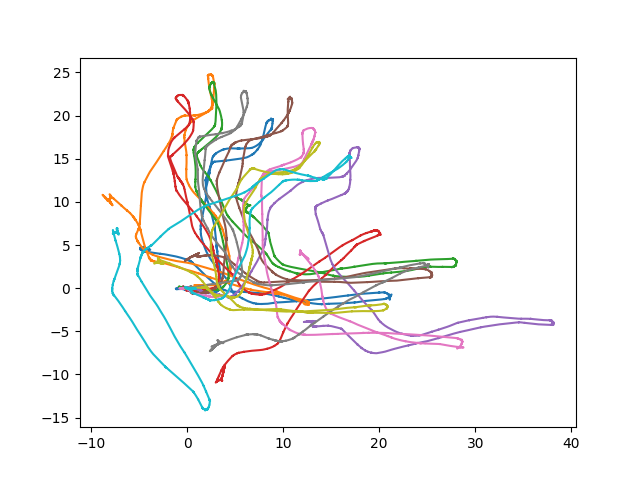
\includegraphics[width=0.5\textwidth]{visualization.png}
    \caption{Visualization of N-Particle motion model}
    \label{fig:N-Particle trajectory}
\end{figure}
\begin{figure}[h]
    \centering
    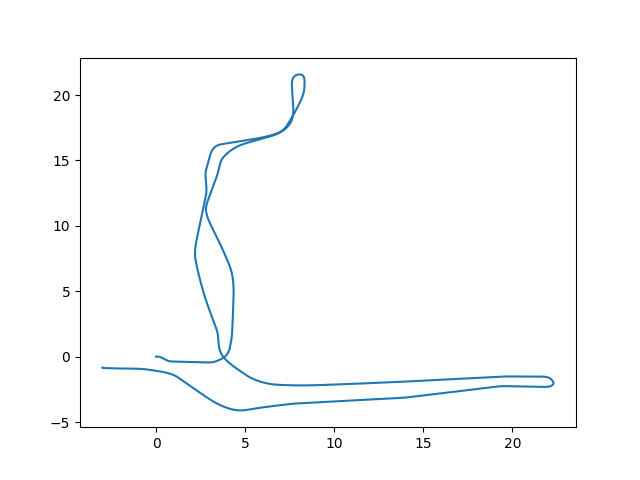
\includegraphics[width=0.5\textwidth]{trajectory.png}
    \caption{Trajectory of the robot}
    \label{fig:trajectory}
\end{figure}
\begin{figure}[h]
    \centering
    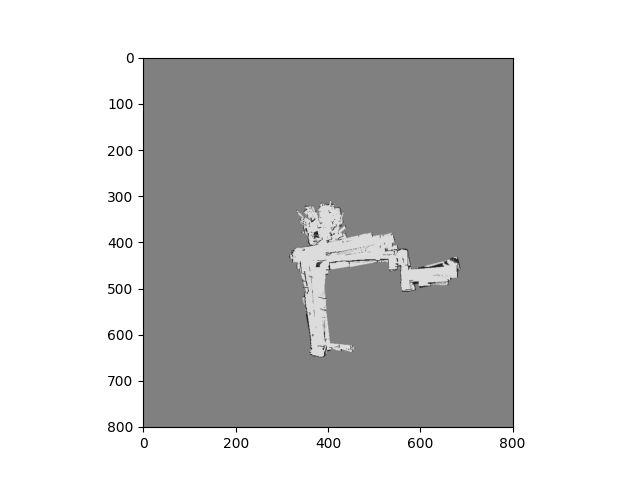
\includegraphics[width=0.5\textwidth]{dead_reckon.png}
    \caption{Occupancy map from dead reckoning}
    \label{fig:occupancy_map}
\end{figure}
\begin{figure}[h]
    \centering
    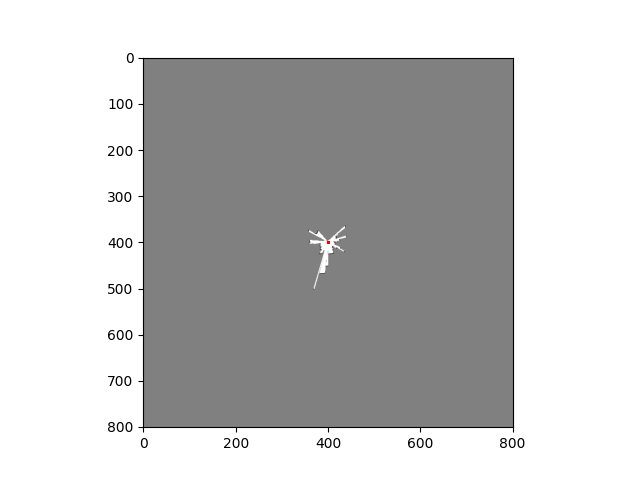
\includegraphics[width=0.5\textwidth]{map0.png}
    \caption{Occupancy map from particle filter}
    \label{fig:particle_filter}
\end{figure}
\begin{figure}[h]
    \centering
    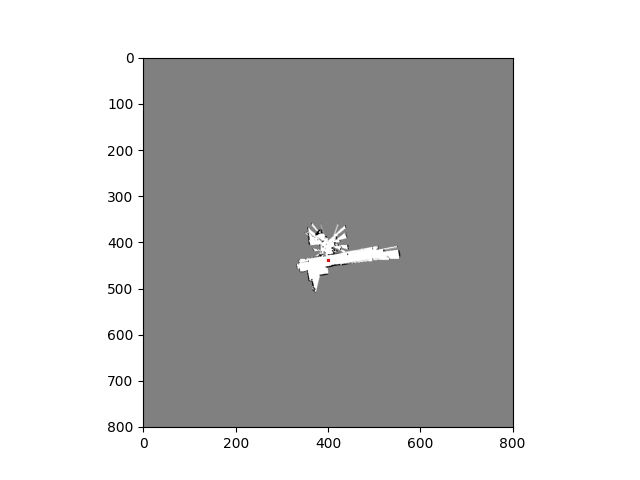
\includegraphics[width=0.5\textwidth]{map800.png}
    \caption{Occupancy map from particle filter}
    \label{fig:particle_filter}
\end{figure}
\begin{figure}[h]
    \centering
    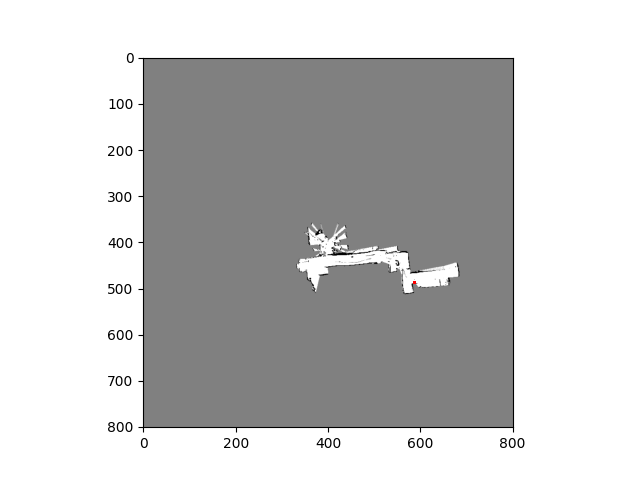
\includegraphics[width=0.5\textwidth]{map1600.png}
    \caption{Occupancy map from particle filter}
    \label{fig:particle_filter}
\end{figure}
\begin{figure}[h]
    \centering
    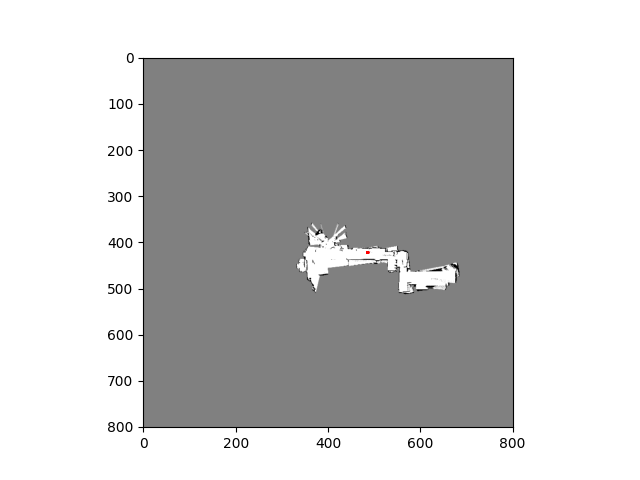
\includegraphics[width=0.5\textwidth]{map2400.png}
    \caption{Occupancy map from particle filter}
    \label{fig:particle_filter}
\end{figure}
\begin{figure}[h]
    \centering
    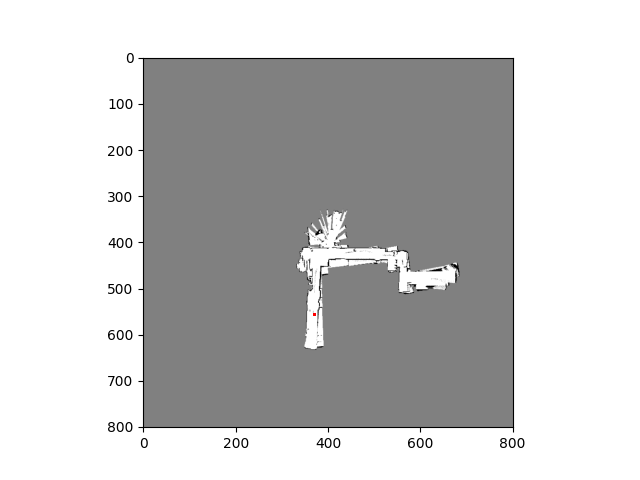
\includegraphics[width=0.5\textwidth]{map3200.png}
    \caption{Occupancy map from particle filter}
    \label{fig:particle_filter}
\end{figure}
\begin{figure}[h]
    \centering
    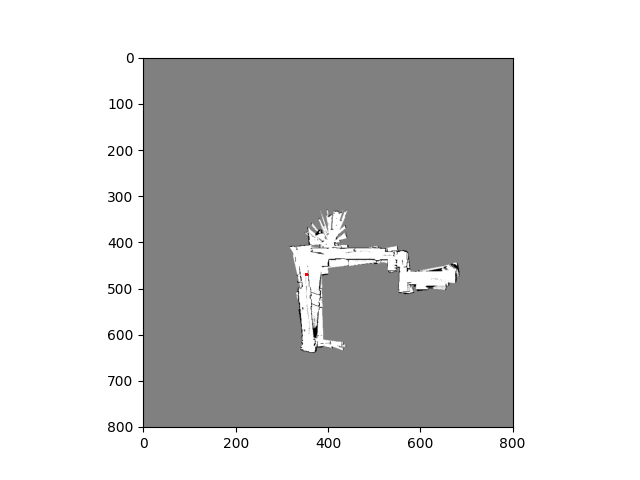
\includegraphics[width=0.5\textwidth]{map4000.png}
    \caption{Occupancy map from particle filter}
    \label{fig:particle_filter}
\end{figure}
\begin{figure}[h]
    \centering
    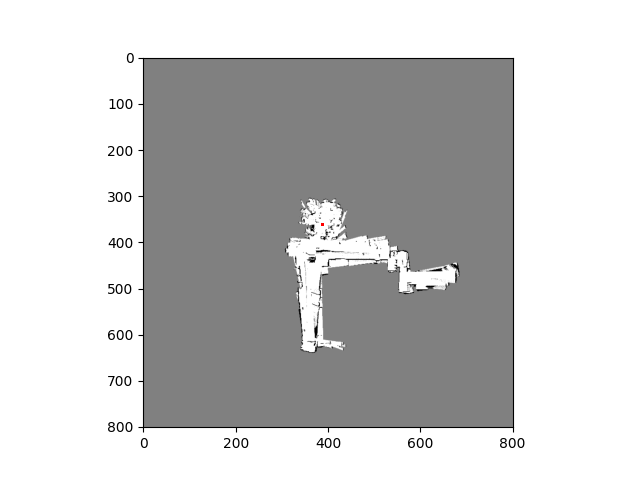
\includegraphics[width=0.5\textwidth]{map4800.png}
    \caption{Occupancy map from particle filter}
    \label{fig:particle_filter}
\end{figure}
\begin{figure}[h]
    \centering
    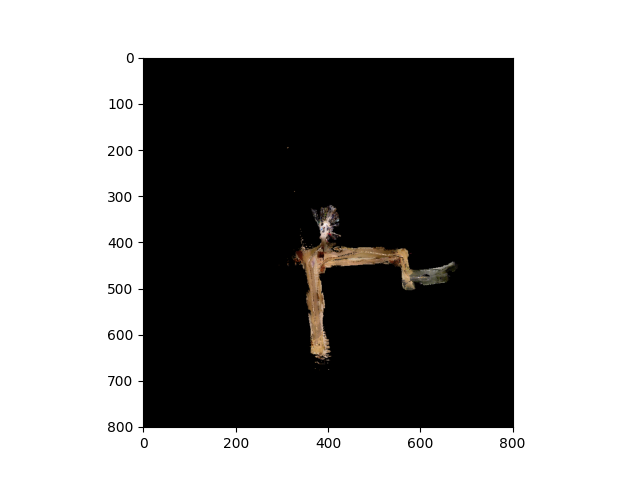
\includegraphics[width=0.5\textwidth]{texture0.png}
    \caption{Occupancy map from particle filter}
    \label{fig:particle_filter}
\end{figure}
\begin{figure}[h]
    \centering
    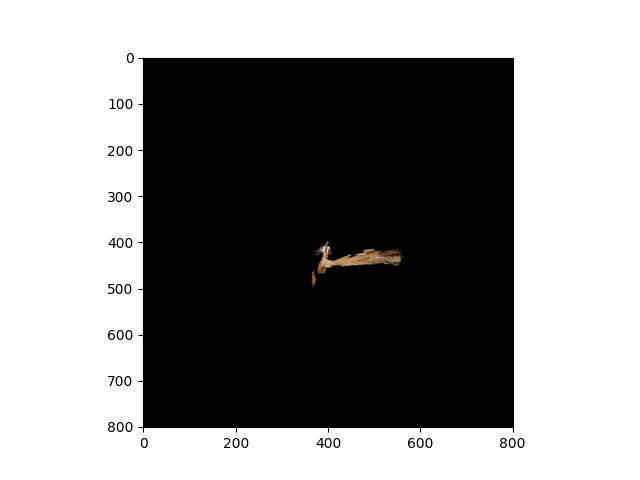
\includegraphics[width=0.5\textwidth]{texture_500.png}
    \caption{Occupancy map from particle filter}
    \label{fig:particle_filter}
\end{figure}
\begin{figure}[h]
    \centering
    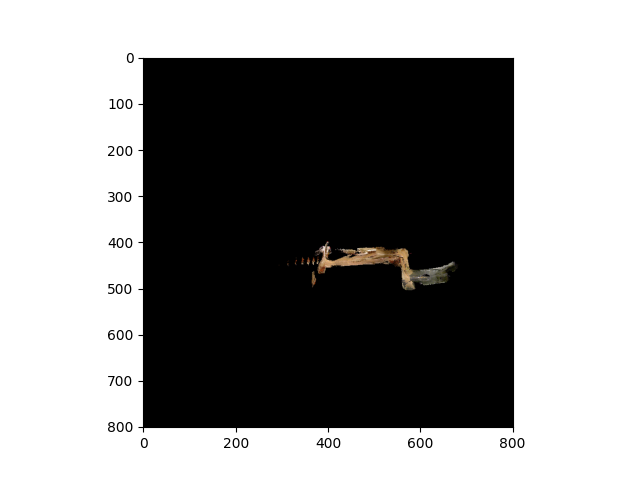
\includegraphics[width=0.5\textwidth]{texture_1000.png}
    \caption{Occupancy map from particle filter}
    \label{fig:particle_filter}
\end{figure}
\begin{figure}[h]
    \centering
    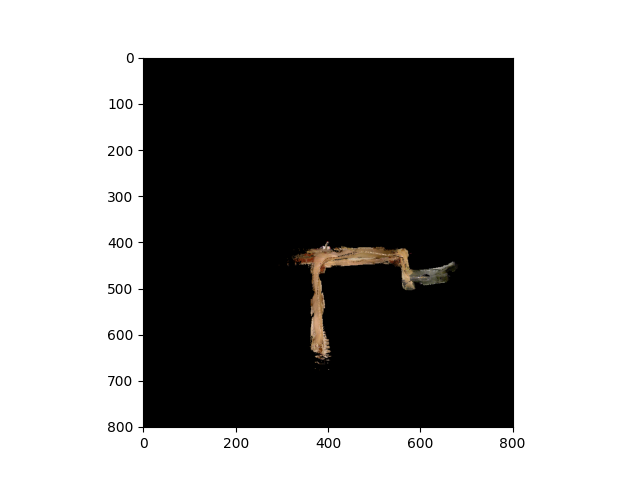
\includegraphics[width=0.5\textwidth]{texture_1500.png}
    \caption{Occupancy map from particle filter}
    \label{fig:particle_filter}
\end{figure}
\begin{figure}[h]
    \centering
    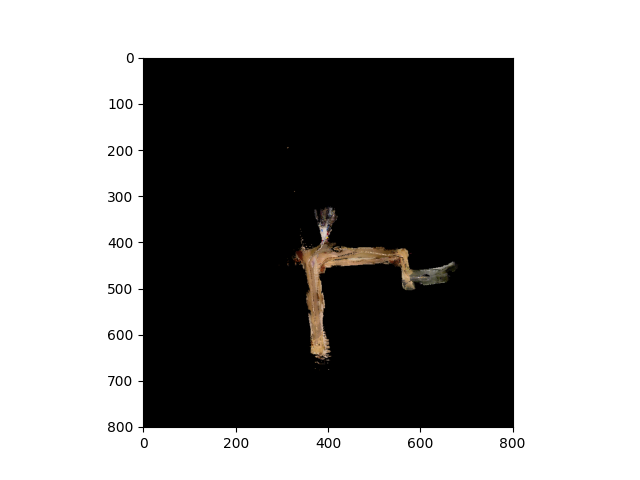
\includegraphics[width=0.5\textwidth]{texture_2000.png}
    \caption{Occupancy map from particle filter}
    \label{fig:particle_filter}
\end{figure}
\subsection{Dataset 21}
\begin{figure}[h]
    \centering
    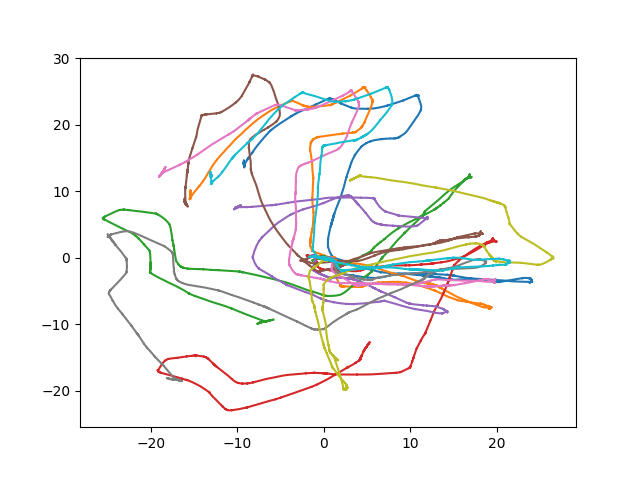
\includegraphics[width=0.5\textwidth]{visualization_1.png}
    \caption{Visualization of N-Particle motion model}
    \label{fig:N-Particle trajectory}
\end{figure}
\begin{figure}[h]
    \centering
    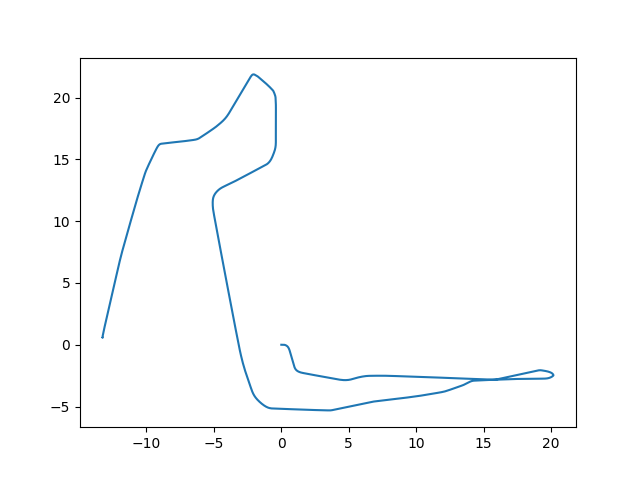
\includegraphics[width=0.5\textwidth]{trajectory_1.png}
    \caption{Trajectory of the robot}
    \label{fig:trajectory}
\end{figure}
\begin{figure}[h]
    \centering
    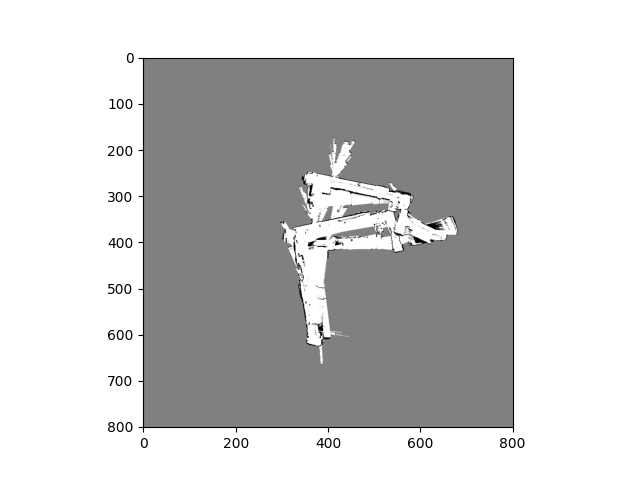
\includegraphics[width=0.5\textwidth]{dead_reckon_1.png}
    \caption{Occupancy map from dead reckoning}
    \label{fig:occupancy_map}
\end{figure}
\begin{figure}[h]
    \centering
    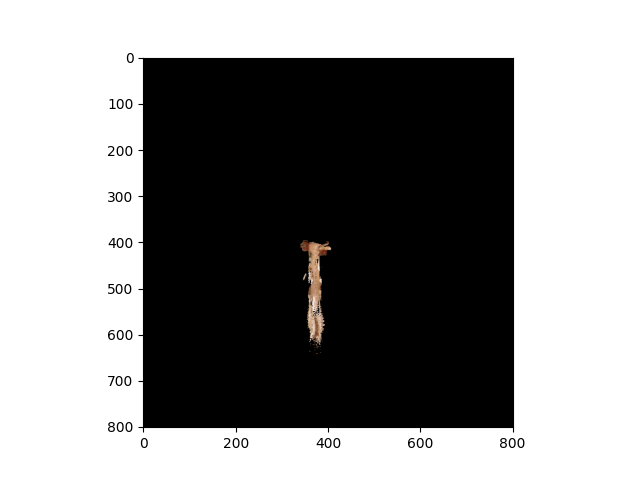
\includegraphics[width=0.5\textwidth]{texture500.png}
    \caption{Occupancy map from particle filter}
    \label{fig:particle_filter}
\end{figure}
\begin{figure}[h]
    \centering
    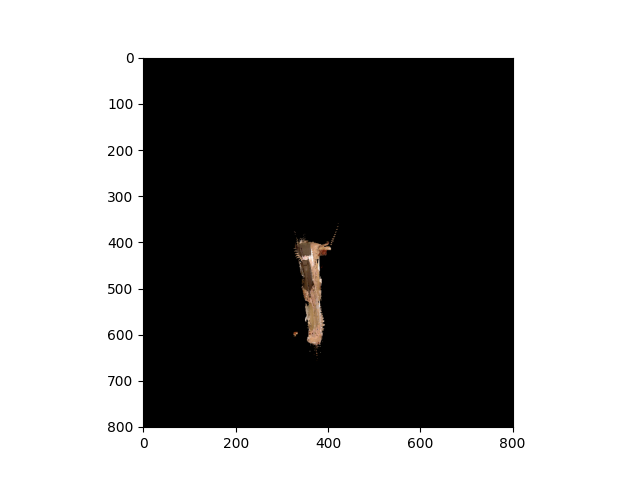
\includegraphics[width=0.5\textwidth]{texture1000.png}
    \caption{Occupancy map from particle filter}
    \label{fig:particle_filter}
\end{figure}
\begin{figure}[h]
    \centering
    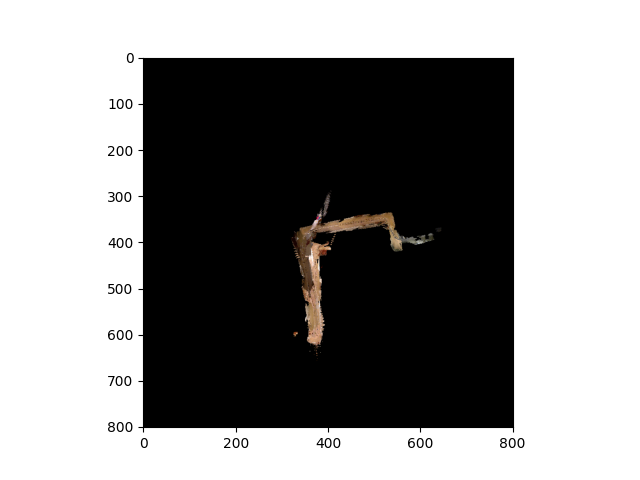
\includegraphics[width=0.5\textwidth]{texture1500.png}
    \caption{Occupancy map from particle filter}
    \label{fig:particle_filter}
\end{figure}
\begin{figure}[h]
    \centering
    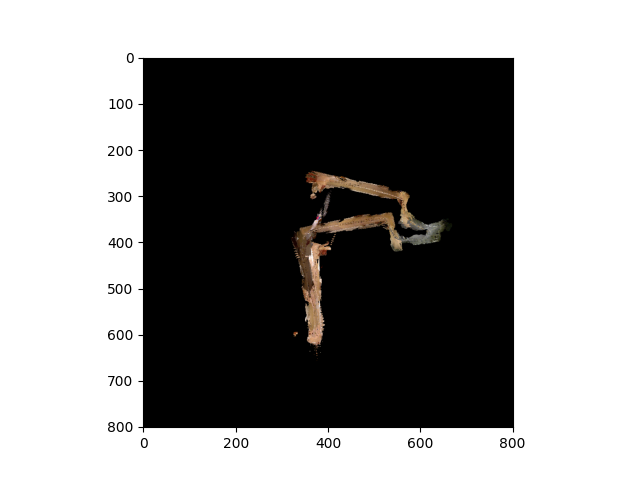
\includegraphics[width=0.5\textwidth]{texture2000.png}
    \caption{Occupancy map from particle filter}
    \label{fig:particle_filter}
\end{figure}
\begin{figure}[h]
    \centering
    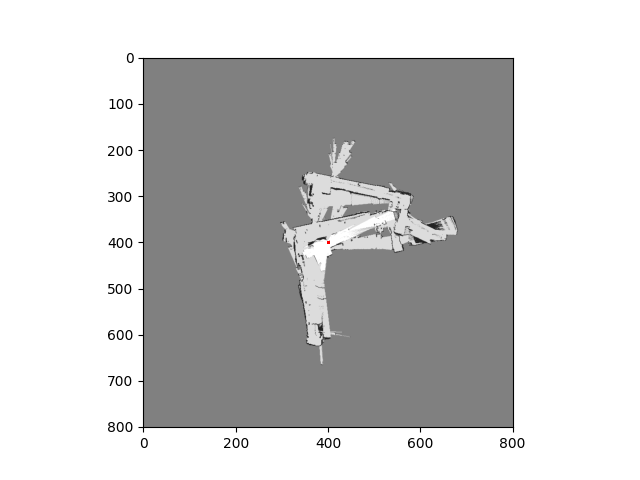
\includegraphics[width=0.5\textwidth]{map_0.png}
    \caption{Occupancy map from particle filter}
    \label{fig:particle_filter}
\end{figure}
\begin{figure}[h]
    \centering
    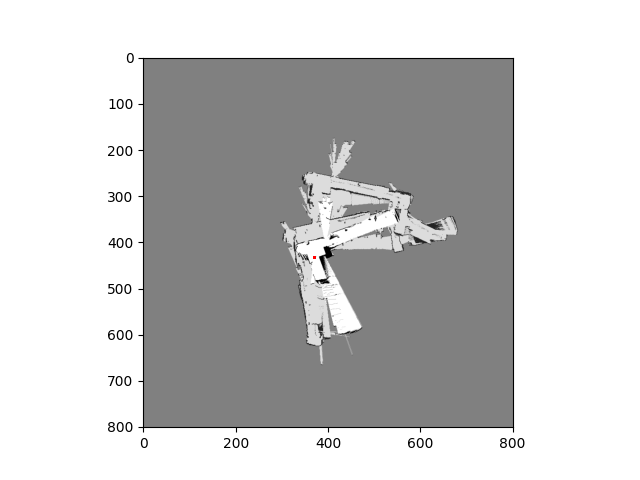
\includegraphics[width=0.5\textwidth]{map_800.png}
    \caption{Occupancy map from particle filter}
    \label{fig:particle_filter}
\end{figure}
\begin{figure}[h]
    \centering
    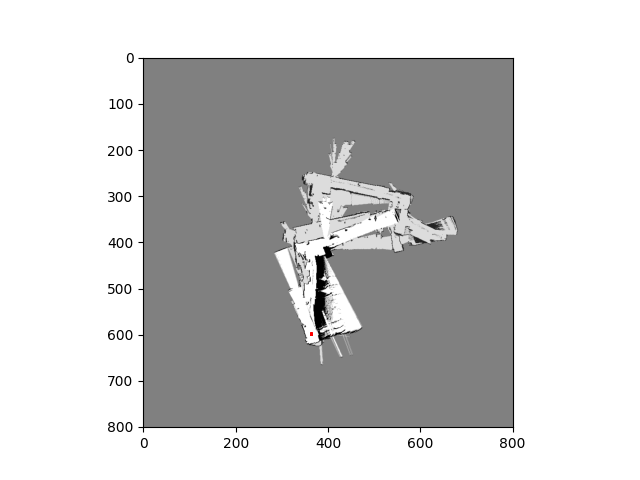
\includegraphics[width=0.5\textwidth]{map_1600.png}
    \caption{Occupancy map from particle filter}
    \label{fig:particle_filter}
\end{figure}
\begin{figure}[h]
    \centering
    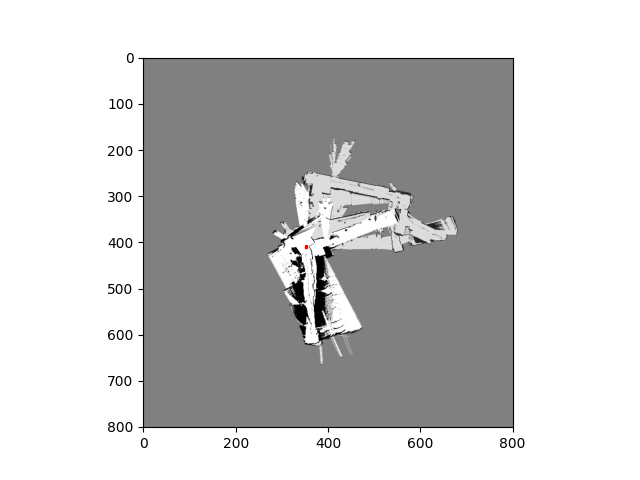
\includegraphics[width=0.5\textwidth]{map_2400.png}
    \caption{Occupancy map from particle filter}
    \label{fig:particle_filter}
\end{figure}
\begin{figure}[h]
    \centering
    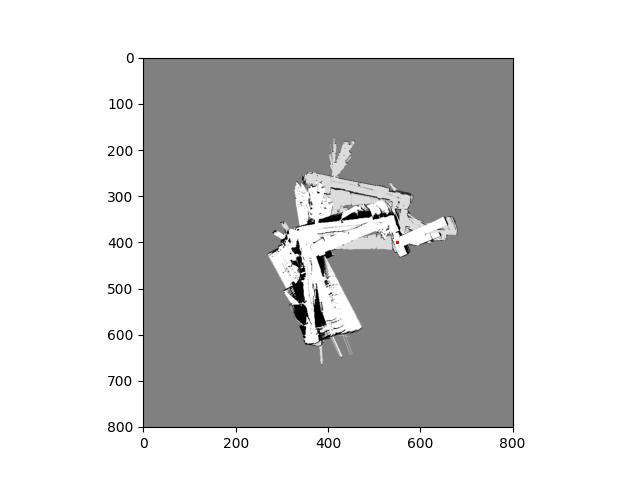
\includegraphics[width=0.5\textwidth]{map_3200.png}
    \caption{Occupancy map from particle filter}
    \label{fig:particle_filter}
\end{figure}
\begin{figure}[h]
    \centering
    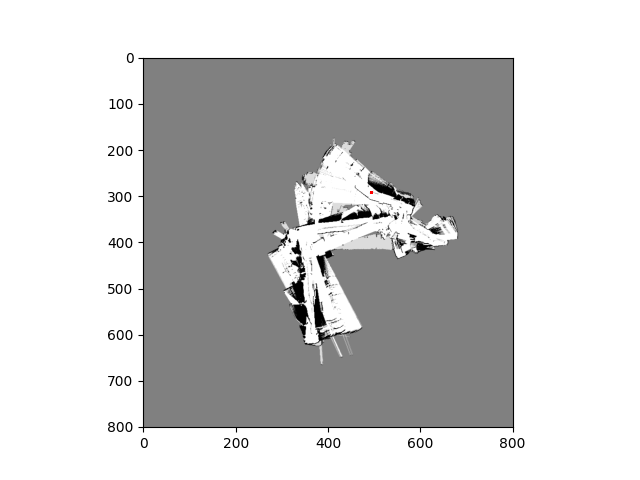
\includegraphics[width=0.5\textwidth]{map_4000.png}
    \caption{Occupancy map from particle filter}
    \label{fig:particle_filter}
\end{figure}
\subsection{Discussion}
\begin{enumerate}
    \item On plotting the robot trajectory using only linear and angular velocity we observed that trajectory in dataset 20 undergoes less drift when compared to dataset 21. So, when we plot the occupancy map using only dead reckon trajectory, we get a better occupancy map for dataset 20 when compared to dataset 21. Hence, ideally particle filter would be helpful in improving the occupancy map for dataset 21.
    \item As mentioned above, the slip in 20 is minor when compared to 21. So, the occupancy map we get when using small number of particles (around 10) is far better in 20 than in 21. To obtain a sensible occupancy map for 21, we needed atleast 50 particles. This is due to the fact that the particles required more exploration to obtain better correlations between the sensor data and the map. Hence, we can increase the exploration for particles by increasing the noise in the system and by increasing the number of particles.
    \item In general, the developed filter is robust to upto 40 percent of noise. The noise here refers to variance in the linear and angular velocity, used in the motion model. If the noise given is more 40 percent of the current velocity, the occupancy grid map could diverge. This can most likely happen when the number of particles is also low. So, if we sample most particles towards an area where map is not developed, most particles will get low correlations (compared to other timesteps) and map could start expanding in undesirable direction.
    \item Currently, while calculating the correlation, we are only perturbing the yaw angle of the particles. This was done to reduce the runtime of the algorithm. We thought that perturbing the yaw angle would be sufficient, since the trajectories of the robot were mostly straight. And slip was only observed while turning. On applying the perturbation along x and y axes we could have generated better results. We can also tune perturbation angle according to our requirements. On a rough road, we need low perturbation angle, as robot would not slip as much as it would on a smooth road. On a smooth road, we can increase the perturbation angle to increase the exploration for correction of pose.
    \item On decreasing the LiDAR likelihood ratio ($\lambda$), we observed that we need more particles to obtain a decent occupancy map. This could be due to the fact that LiDAR data did not have much noise since it was recorded indoors (figured from the images).
    \item The threshold for resampling of the particles (mentioned above) was chosen by trial and error. Intuition behind this was, we are starting with a uniform distribution of weights for all particles, when particle reaches the weight (< 25\% of the initially assigned weight), it was not able to able improve even at the later timesteps. So, it was better discard that particle as we were not able to explore efficiently.
    \item One of major error done during the project was to assume that LiDAR and encoders readings are synchronized. This resulted in a lot of drift in the occupancy map.
    \item The procedure of texture mapping was straight forward and we were able to obtain decent results. Although, we were not able to figure out the use of the texture map. As the generated texture map was not very clear due to small width of the path.
\end{enumerate}
\end{document}